\section{Оценка неопределённости для байесовской оптимизации.}

\subsection*{Гауссовский процесс}

\D{
    Стохастический процесс (совокупность случайных величин),
    т.ч. любая конечная линейная комбинация из них нормально
    распределена.

    Задается ковариационной функцией.
}

Используется в качестве суррогатной функции.

Получение предсказания:
\begin{itemize}
    \item $k$ - ковариационная функция, $x_i$ - объект тренировочного
    набора, $y_i$ - значение целевого признака.
    \item $K_{i, j} = k(x_i, x_j)$ - ковариационная матрица.
    \item $k(x')$ - вектор ковариаций запроса с объектами тренировочной выборки.
    $k_i(x') = k(x_i, x')$
    \item $\mu(x') = k(x') \times K^-1 \times y$ - предсказание.
    \item $\sigma^2(x') = k(x', x') - k(x') \times K^-1 \times k(x')$ - дисперсия.
    \item $K^-1$ не зависит от запроса, можно предпосчитать.
    \item Если в данных есть шум с дисперсией $\tau$, то
    $K^-1 \to (K + \tau I)^-1$
\end{itemize}

Ковариационные функции:
\begin{itemize}
    \item $C$
    \item $\langle a, b \rangle$
    \item $exp\left(- 1/2 \cdot (a - b) \times \Theta^-2 \times (a - b)\right)$,
    где $\Theta$ - масштабирующая матрица
\end{itemize}

Можно определить как выбор подмножества функций, проходящих через
известные точки.

\subsection*{Ансамбль моделей}

Множество моделей: $a_1, ..., a_T$

Ответ ансамбля: $y(x) = \mathbb{E}[a_i]$

Дисперсия предсказания: $\sigma^2(x) = \mathbb{D}[a_i(x)]$

Подходит случайный лес. Деревья в целом классные для ансамблирования
(быстрые, легкие). Но плохо экстраполирует функцию (края особенно).

\subsection*{Нейронки}

Берем дропаут и, вместо отключения на тесте, оставляем его,
сэмплируем ответ и считаем дисперсию.

% \begin{figure}[H]
% 	\centering
% 	\begin{minipage}[b]{0.4\textwidth}
% 		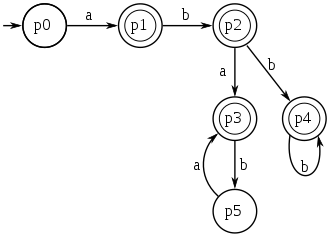
\includegraphics[width=\textwidth]{images/dfa.png}
% 		\caption{Пример графа переходов детерминированного КА.}
% 	\end{minipage}
% 	\hfill
% 	\begin{minipage}[b]{0.4\textwidth}
% 		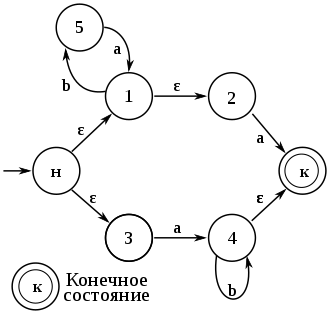
\includegraphics[width=\textwidth]{images/ndfa.png}
% 		\caption{Пример графа переходов недетерминированного КА с самопроизвольными переходами.}
% 	\end{minipage}
% \end{figure}